\documentclass[titlepage]{article}

\usepackage{booktabs}
\usepackage{tabularx}
\usepackage{graphicx}
\usepackage[left=2cm, right=2cm, top=2cm, bottom=2cm]{geometry}
\usepackage{float}

\title{Development Plan\\\progname}

\author{\authname}

\date{}

%% Comments

\usepackage{color}

\newif\ifcomments\commentstrue %displays comments
%\newif\ifcomments\commentsfalse %so that comments do not display

\ifcomments
\newcommand{\authornote}[3]{\textcolor{#1}{[#3 ---#2]}}
\newcommand{\todo}[1]{\textcolor{red}{[TODO: #1]}}
\else
\newcommand{\authornote}[3]{}
\newcommand{\todo}[1]{}
\fi

\newcommand{\wss}[1]{\authornote{blue}{SS}{#1}} 
\newcommand{\plt}[1]{\authornote{magenta}{TPLT}{#1}} %For explanation of the template
\newcommand{\an}[1]{\authornote{cyan}{Author}{#1}}

%% Common Parts

\newcommand{\progname}{Mechatronics Engineering} % PUT YOUR PROGRAM NAME HERE
\newcommand{\authname}{Team 10, LiDart
\\ Jonathan Casella
\\ Karim Elmokattaf
\\ Michaela Schnull
\\ Neeraj Ahluwalia} % AUTHOR NAMES                  

\usepackage{hyperref}
    \hypersetup{colorlinks=true, linkcolor=blue, citecolor=blue, filecolor=blue,
                urlcolor=blue, unicode=false}
    \urlstyle{same}
                                


\begin{document}

\maketitle

\newpage

\begin{table}[hp]
\caption{Revision History} \label{TblRevisionHistory}
\begin{tabularx}{\textwidth}{llX}
\toprule
\textbf{Date} & \textbf{Developer(s)} & \textbf{Change}\\
\midrule
26/Sep/2022 & Michaela Schnull & Initial Release\\
\bottomrule
\end{tabularx}
\end{table}

\begin{table}[hp]
\caption{Acronyms} \label{Acronyms}
\begin{tabularx}{\textwidth}{lX}
\toprule
\textbf{Acronym} & \textbf{Description} \\
\midrule
API & Application Programming Interface \\
CAD & Computer Aided Design\\
CI & Continuous Integration\\
LIDAR & Light Detection and Ranging\\
PR & Pull Request\\
UI & User Interface\\
UX & User Experience\\
\bottomrule
\end{tabularx}
\end{table}

\newpage

\section{Introduction}

3D scanning is a versatile technology that is used across many industries, but its uses are often limited by high cost and complexity. LiDart aims to build a low cost, simple to use 3D scanning robot. A software suite will process data obtained from the robot and provide a user interface. LiDart's end product will be a wheel based mobile robot with all required sensors on-board that can be connected to over WiFi.

\section{Team Meeting Plan}

Weekly meetings will take place in H.G. Thode Library of Science and Engineering. During in-person meetings, our group will review issues tracked on the GitHub project board and identify actions to be taken. The frequency of meetings is subject to change depending the needs of the project. 

\section{Team Communication Plan}

The team will use instant messaging for items that require and urgent response. Communication will also occur through GitHub using issues. Users will be tagged in issues that require their attention. All team members members may schedule  meetings to address specific issues. 

\section{Team Member Roles and Responsibilities}

\subsection{Jonathan Casella}
\begin{itemize}
\item Development and implementation of computer vision algorithms
\item Development and implementation of localization algorithms
\item Creation of a user application that displays the scanning data
\end{itemize}

\subsection{Karim Elmokattaf}
\begin{itemize}
\item Development of the controls software for the robot
\item Development and implementation of localization algorithms
\item Interfacing of hardware and software systems
\item UI/UX design of a user application that displays the scanning data
\end{itemize}

\subsection{Michaela Schnull}
\begin{itemize}
\item Electrical design of the robot, including the creation of electrical schematics to document electrical design
\item Interfacing of hardware and software systems
\item Project management activities, including maintenance of the project board on GitHub, budgeting, scheduling, and acting as the team liaison
\end{itemize}

\subsection{Neeraj Ahluwalia}
\begin{itemize}
\item Mechanical design of the robot, including the creation of CAD models
\item Interfacing of electrical components in the mechanical design
\item Marketing activities, including logo design and video presentations
\end{itemize}

\section{Workflow Plan}

\subsection{GitHub Development Workflow}

The workflow depicted in Figure~\ref{fig:Workflow} will be followed throughout the development process. This workflow supports CI and issue tracking trough GitHub. Commits should be frequent and have descriptive messages.

\begin{figure} [H]
\begin{center}
	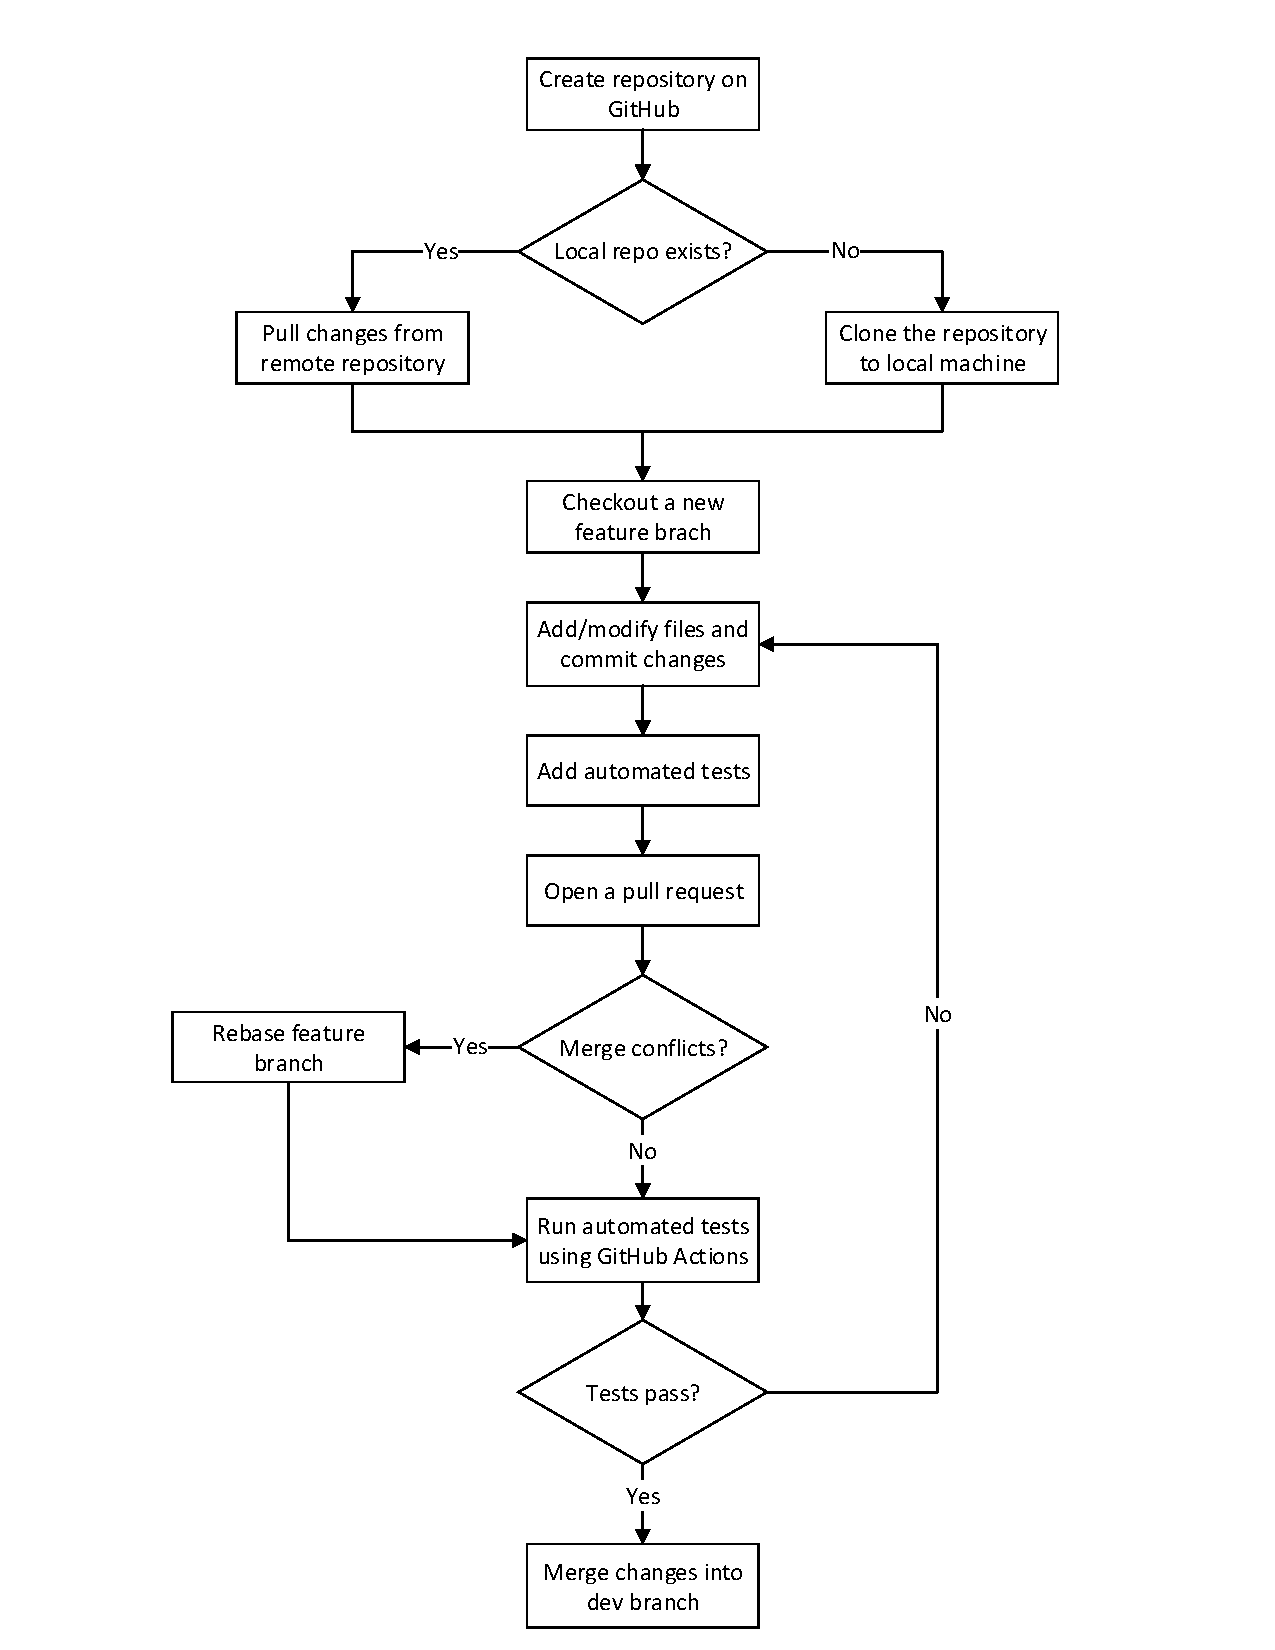
\includegraphics [width=0.8\textwidth] {Figures/GitHub Workflow.pdf}
	\caption{GitHub Development Workflow}
	\label{fig:Workflow}
	\end{center}
\end{figure}

\subsection{Branches}

Development will take place on a development (dev) branch. Feature branches will be used to fix bugs and add new features. They will be deleted after merging into the dev branch.  Changes from the dev branch will be merged to the main branch after they have been reviewed and integration testing has been performed. Figure~\ref{fig:Branches} depicts a sample branching structure.

\begin{figure} [H]
\begin{center}
	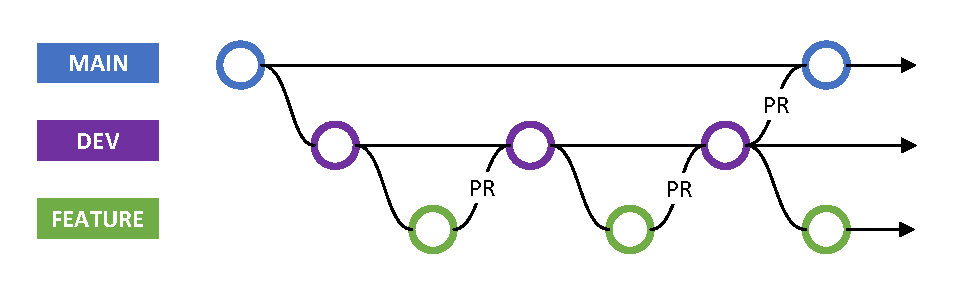
\includegraphics [width=0.8\textwidth] {Figures/GitHub Branches.pdf}
	\caption{Simple Branching Structure}
	\label{fig:Branches}
	\end{center}
\end{figure}

\subsection{Issue Tracking}

GitHub issues will be used to plan and track tasks. All team members can create new issues and assign them to team members. The following guidelines will be followed when working with issues:

\begin{itemize}
\item Issue templates will be used for bug reports and new feature requests
\item Issues that require multiple steps should include task lists
\item Default labels provided by GitHub will be used to classify the type of issue
\item Issues should be linked to associated branches
\end{itemize}

A GitHub project board will be used to track and organize issues. Issues will be sorted into \textit{Todo}, \textit{In Progress}, and \textit{Done} columns in a tabular view. Furthermore, issues will be assigned fields to categorize them based on priority and discipline. The priority field will classify issues as \textit{High}, \textit{Medium}, or \textit{Low} priority. The discipline field will classify issues as \textit{Mechanical}, \textit{Electrical}, or \textit{Software}.

\section{Proof of Concept Demonstration Plan}

\subsection{Inaccurate Localization}
Indoor robot localization is a complex and challenging problem.
The robot must be able to determine its position using image based camera localization. Challenges associated with this include probabilistic sensor data,sensor aliasing, noise in image, an geometric characteristics of surrounding environment. The machine vision algorithms will be developed and tested using images taken from a phone camera. The localization algorithm will determine the position of the phone from the images taken.

\subsection{Low Accuracy of LIDAR Scans}

The LIDAR sensor that will be used on the robot will be procured and tested. The LIDAR sensor will be used to scan a known object. The data obtained will be run through a program that displays the scanning data. This data will be compared to the known object to determine the accuracy of the sensor.

\subsection{Robot Mechanical and Electrical Design}

The robot must be able to move around and position itself. A prototype of the robot will be created to prove the electrical and mechanical design concepts. The robot should be able to follow simple movement commands.

\section{Technology}

\begin{itemize}
\item Autodesk Inventor: CAD tool used to develop and model the mechanical design of the robot
\item AutoCAD Electrical: CAD tool used to create electrical schematics
\item Autodesk EAGLE: CAD tool used to design printed circuit boards
\item Rust: High performance, low-level programming language ideal for embedded systems with built-in unit-testing
\item Rustfmt: Lint tool designed for the Rust programming language
\item OpenGL: API used to render scanning data
\item OpenCV: Real-time computer vision library 
\item AprilTags: Visual marker system designed for use in robotics and camera calibration
\item GitHub: Version control software with tools for CI and project management

\end{itemize}

\section{Coding Standard}

The \textit{Rust Style Guide} will be used as a coding standard.

\section{Project Scheduling}

\begin{figure} [H]
\begin{center}
	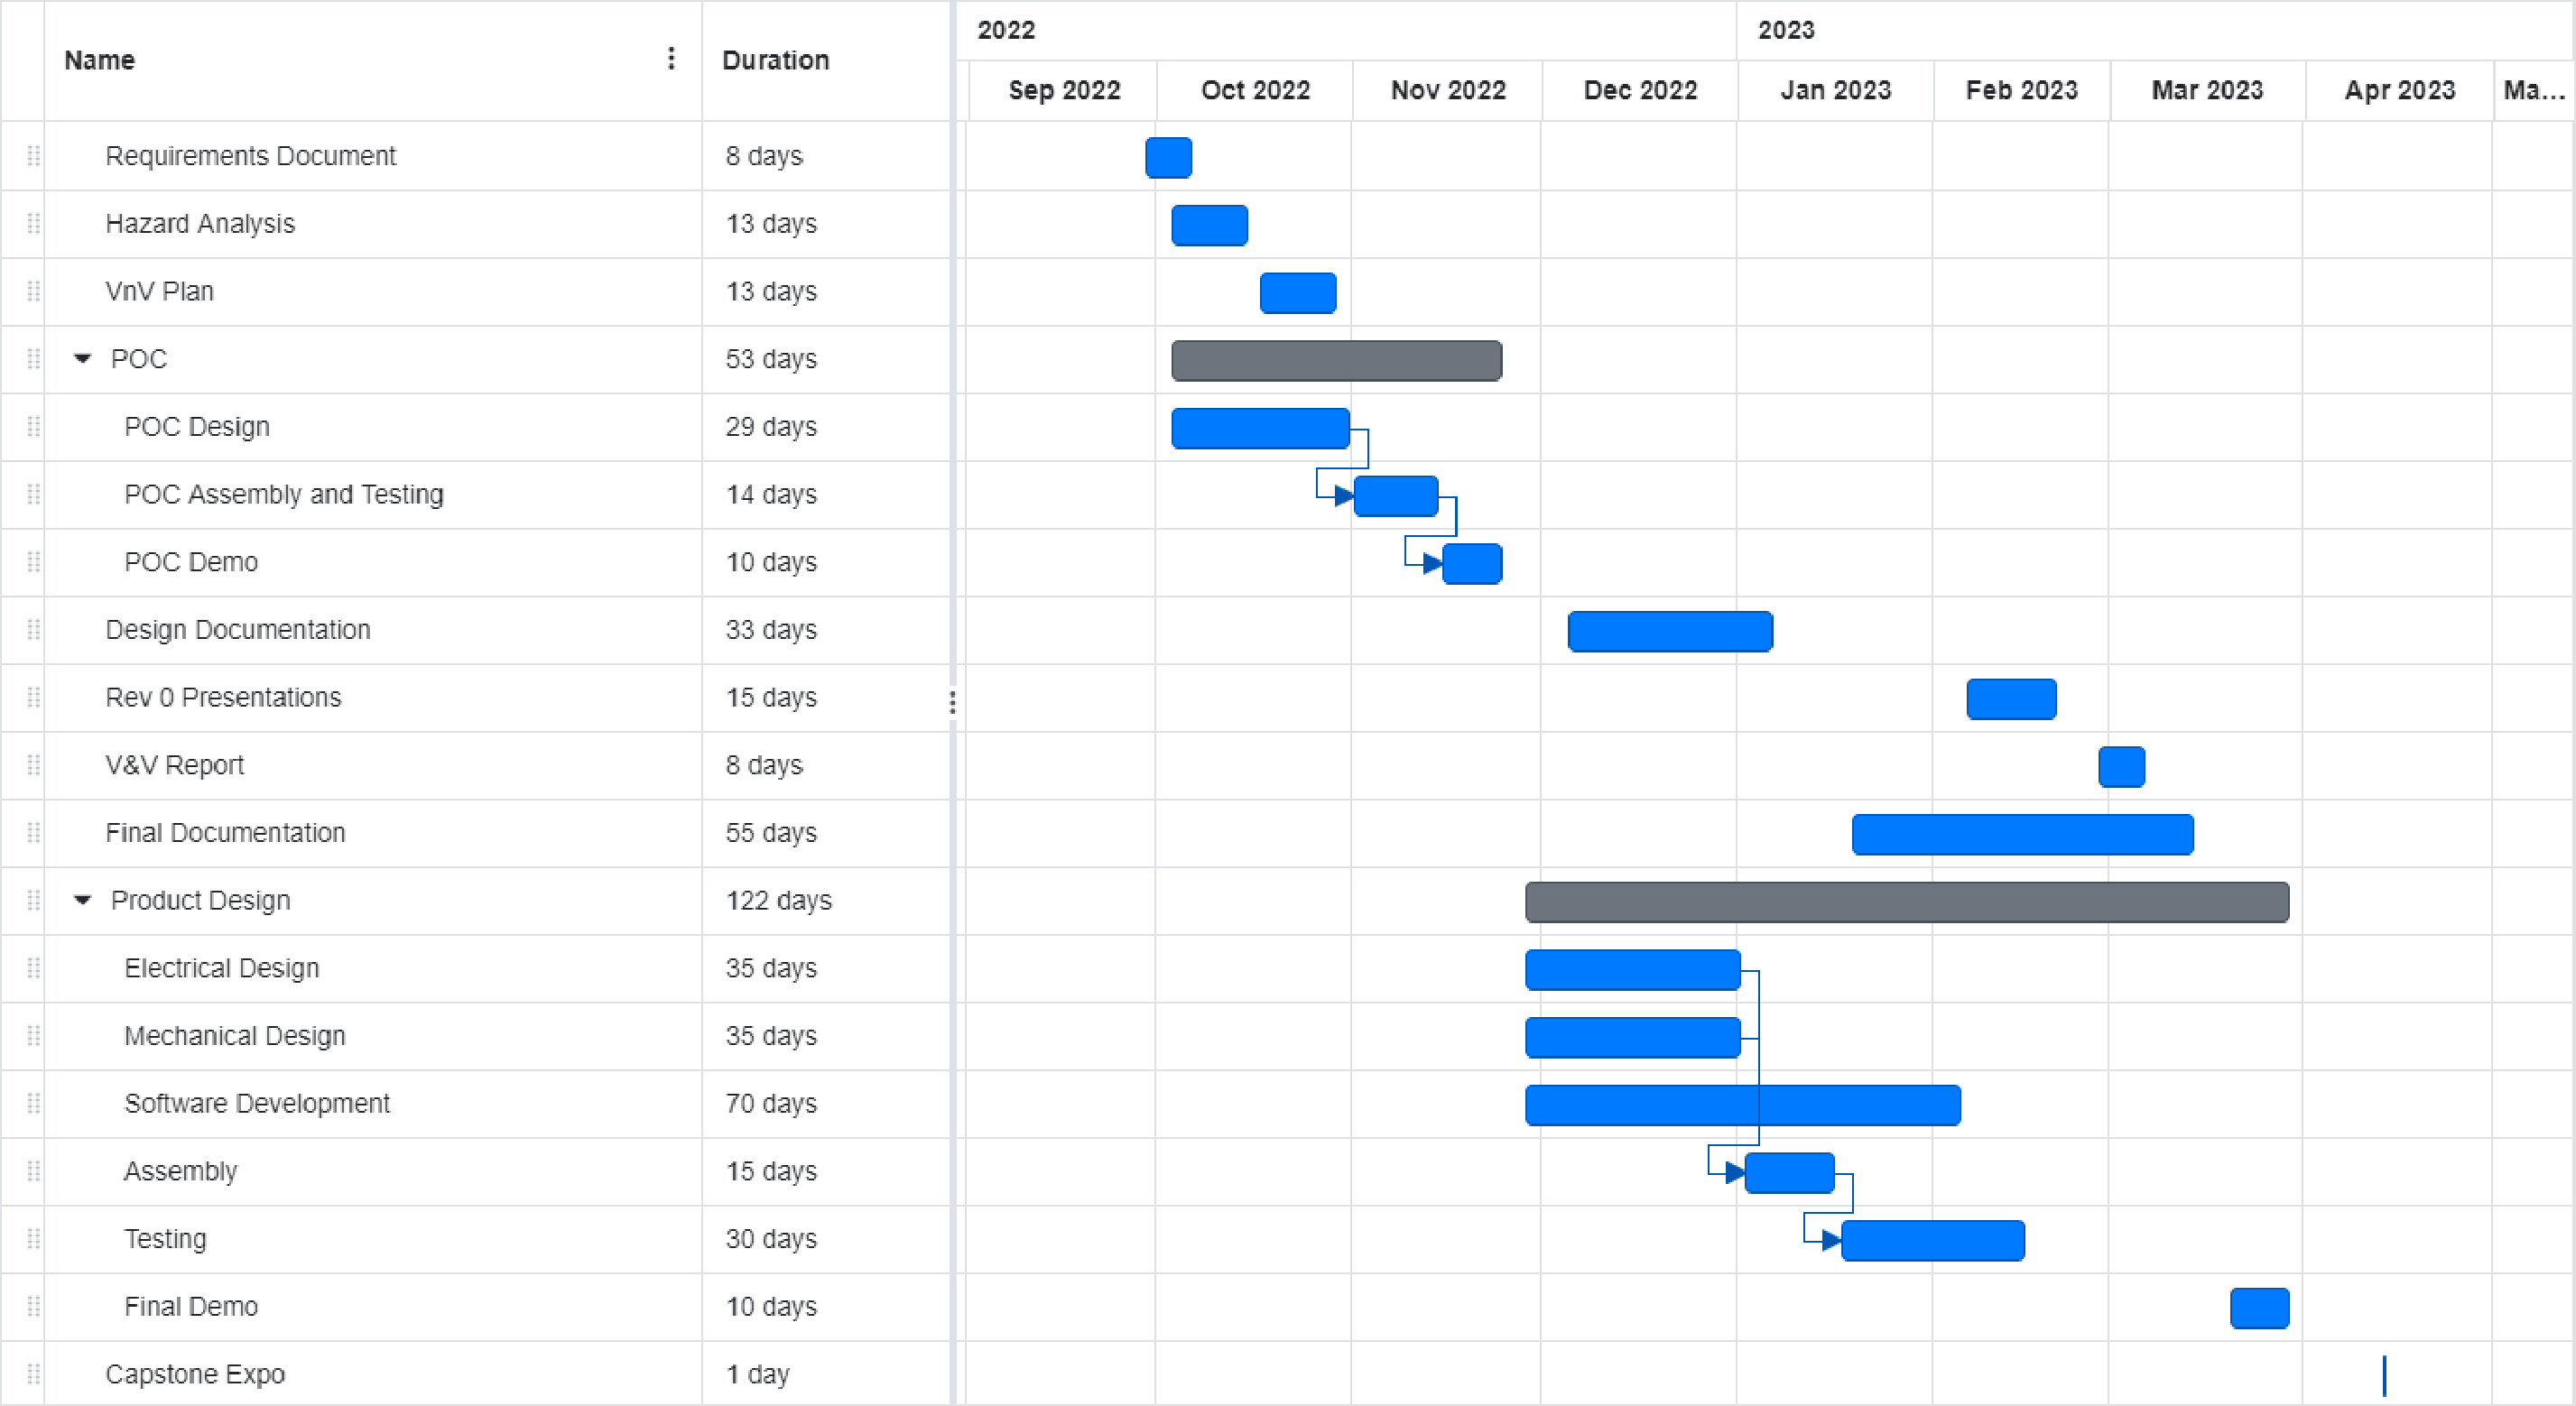
\includegraphics [width=1\textwidth] {Figures/Gantt.pdf}
	\caption{Gantt Chart}
	\label{fig:Gantt}
	\end{center}
\end{figure}

\end{document}